\documentclass{article}
\usepackage{graphicx}
\usepackage{nopageno}
\usepackage{txfonts}
\usepackage[usenames]{color}
\usepackage[T2A]{fontenc}
\usepackage[utf8]{inputenc}
%\usepackage{amsmath}

\begin{document}
\begin{center}
	\begin{figure}[htbp] %  figure placement: here, top, bottom, or page
	   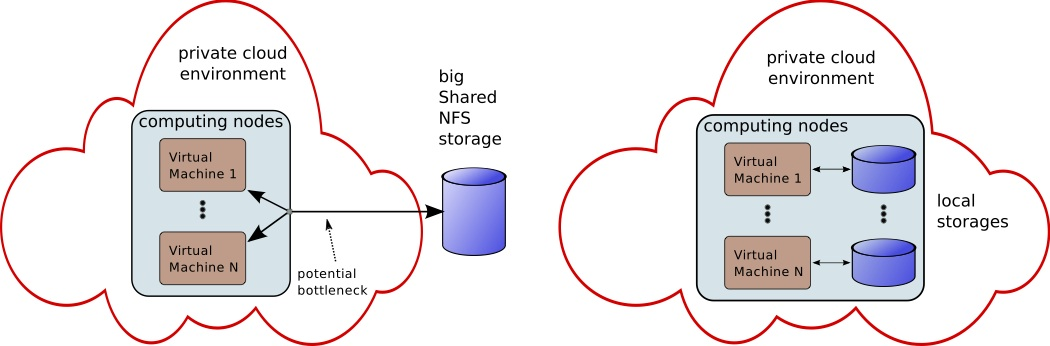
\includegraphics[width=13cm]{fig3.jpg} 
	   \caption{Sketch of difference between the possible scenarios of Hadoop deployment: Shared~TM and SSH~TM. The Shared~TM deployment scenario (left) assumes that the storage, where the data is being keeped and proceeded, is a NFS-mounted Shared Storage, connected to the computing nodes by a fast cable. The SSH~TM (right) is in opposite engages the local storages of each virtual node, which are usually not slower than a fast cable. The difference emerges then computation nodes start to communicate with each other in order to share with the data. In that case, even fast cable starts to saturate, and the IO bottleneck appears.}
	   \label{fig:fig3}
	\end{figure}
\end{center}
\end{document}
